\section{Showing the structure of \loglin{} models}\label{sec:mosaic-struc}
The mosaic display can also be used to illuminate the relations among
variables in a \ctab{} which are represented in various \loglin{} models,
a point described by \citet{TheusLauer:99}.
Each of the model types depicted in \tabref{tab:hyp3way} has, in fact,
a characteristic shape and structure in a mosaic display. This,
in turn, leads to a clearer understanding of the structure which appears
in real data when a given model fits, the relations among the models,
and the use of mosaic displays.

%%
%% Table struc written by md2tex 29MAY98 08:46
%%
\begin{table}[htb]
 \caption{A $2 \times 2 \times 2$ table (artificial data)}
 \label{tab:struc}
 \begin{center}
  \begin{tabular}{|l|rrrr|r|}
   \hline
% & \multicolumn{4}{c|}{\bfseries\large B} & \rule{0in}{2.5ex}\\
 & \multicolumn{2}{c|}{B1} & \multicolumn{2}{c|}{B2} &  \\\cline{2-5}
% & \multicolumn{4}{c|}{\bfseries\large A} & \rule{0in}{2.5ex}\\
{\bfseries\large C} & A1 & A2 & A1 & A2& {\bfseries\large Total} \\
   \hline
C1   &     6 &    10 &   312 &    44 &   372 \\
C2   &    37 &    31 &   192 &    76 &   336 \\
   \hline
\rule{0in}{2.5ex}{\bfseries\large Total} &   43 &    41 &   504 &   120 &   708 \\
   \hline
  \end{tabular}
 \end{center}
\end{table}

To show this, we use artificial data for a $2 \times 2 \times 2$ table
shown in \tabref{tab:struc}.
We can force such a table to conform to any \loglin{} model
(e.g., $H_1$ -- $H_4$)
simply by finding the expected frequencies under that model
and constructing a mosaic depicting the expected frequencies.

\subsection{Mutual independence}
For example, to show the structure of a table which fits
mutual independence, $H_1$, use the \FUNC{IPF} to find the
fitted values, \texttt{fit}, as

\begin{verbatim}
proc iml;
   table = { ... };
   dim= {2 2 2};
   vnames={A B C};
   lnames = {'A1' 'A2',  'B1' 'B2',  'C1' 'C2'};

   config = {1 2 3};
   call ipf(fit,status,dim,table,config);
   fittype='MUTUAL';
   print fittype config[f=4.] fit[f=7.2];
\end{verbatim}
The fitted frequencies then have the same one-way margins as the
data in \tabref{tab:struc}, but have no two-way or higher associations.
We then display a mosaic for the \emph{fitted frequencies}
to see what mutual independence looks like in a three-way table.
\begin{output}
   FITTYPE  CONFIG             FIT
   MUTUAL      1   2   3     34.10   10.04  253.31   74.56
                             30.80    9.07  228.79   67.34
\end{output}
What you see in a mosaic display depends, in large measure, on the order in
which the table variables are entered.
For three variables there are $3!=6$ possible orders;  conveniently,
they are all shown in the mosaic matrix.
In this display we show the three-way mosaic (\texttt{plots=3;})
for each pair of variables, using the fitted values as the ``data.''
The statements below produce \figref{fig:mosfit-1}.
\begin{figure}[htb]
  \centering
  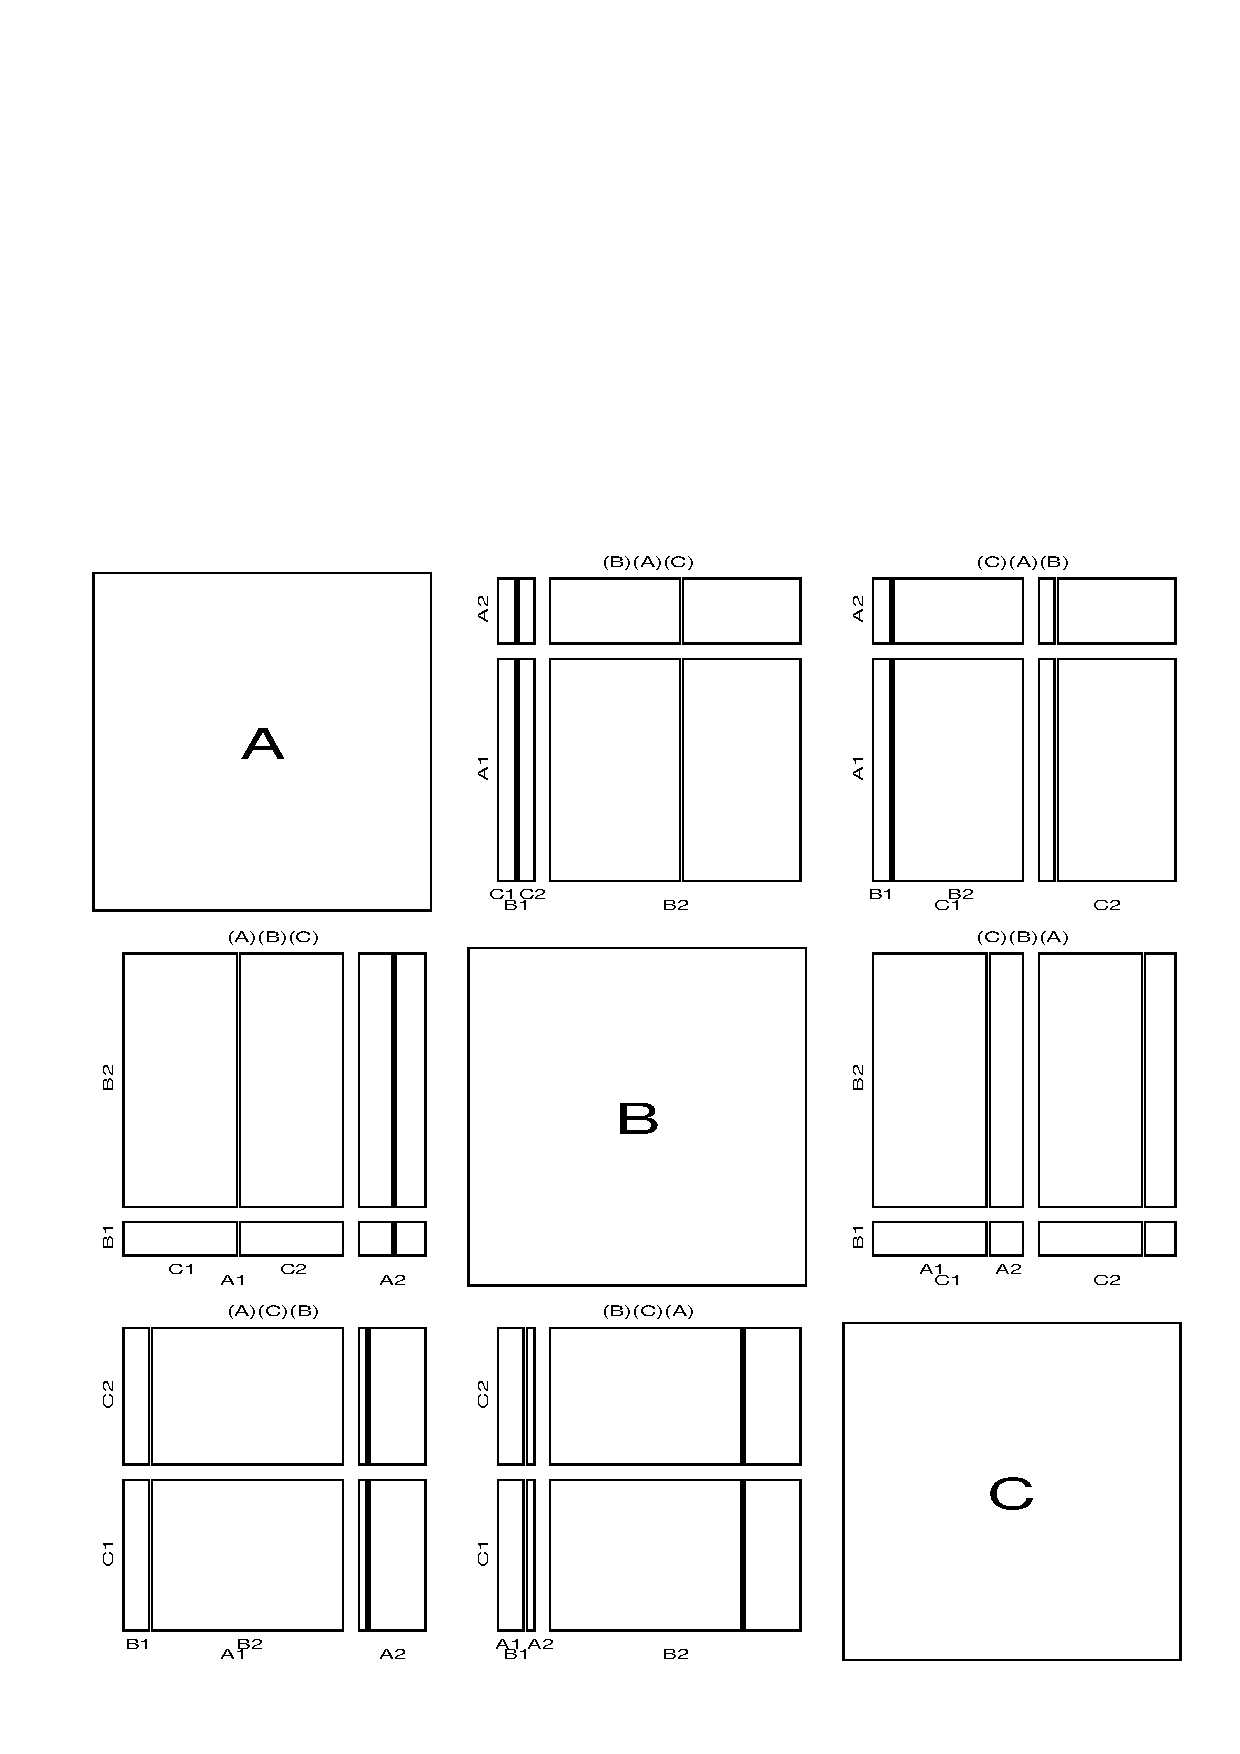
\includegraphics[scale=.6]{ch4/fig/mosfit-1}
  \caption[Mosaic matrix for mutual independence]{Mosaic matrix for mutual independence.  All panels show marginal and conditional independence among all three pairs of variables.}%
  \label{fig:mosfit-1}
\end{figure}

\begin{verbatim}
   plots=3;
   title=fittype+'&MODEL';
   space={12 5};
   run mosmat(dim, fit, vnames, lnames, plots, title);
quit;
%panels(rows=3, cols=3, equate=Y, order=down);
\end{verbatim}


In this figure the same data are shown in all the off-diagonal panels
and the mutual independence model was fitted in each case, but with the
table variables permuted.  All residuals are exactly zero in all cells,
by construction.
We see that in each view, the four large
tiles, corresponding to the first two variables align, indicating
that these two variable are marginally independent.
For example, in the $(1,2)$ panel, $A$ and $B$ are independent, collapsed
over variable $C$.

Moreover, comparing the top half to the bottom half
in any panel we see that the divisions by the third variable
are the same for both levels of the second variable.
In the $(1, 2)$ panel, for example, $A$ and $C$ are independent at
$B1$, and also independent at  $B2$.
This means, though, that $A$ and $B$ are conditionally independent
given $C$ ($A \perp B \given C$).
Because this holds in all six panels, we see that mutual independence
is equivalent to \emph{all pairs} of variables being conditionally
independent, given the remaining one,  ($X \perp Y \given Z$) for all
permutations of variables.

\subsection{Joint independence}
The model of joint independence, $H_2: \: (A, B) \perp C$, or
equivalently, the \loglin{} model $[A B][C]$
may be visualized similarly by the mosaic matrix in \figref{fig:mosfit-21},
in which the data were replaced by fitted values under this model.
\begin{figure}[htb]
  \centering
  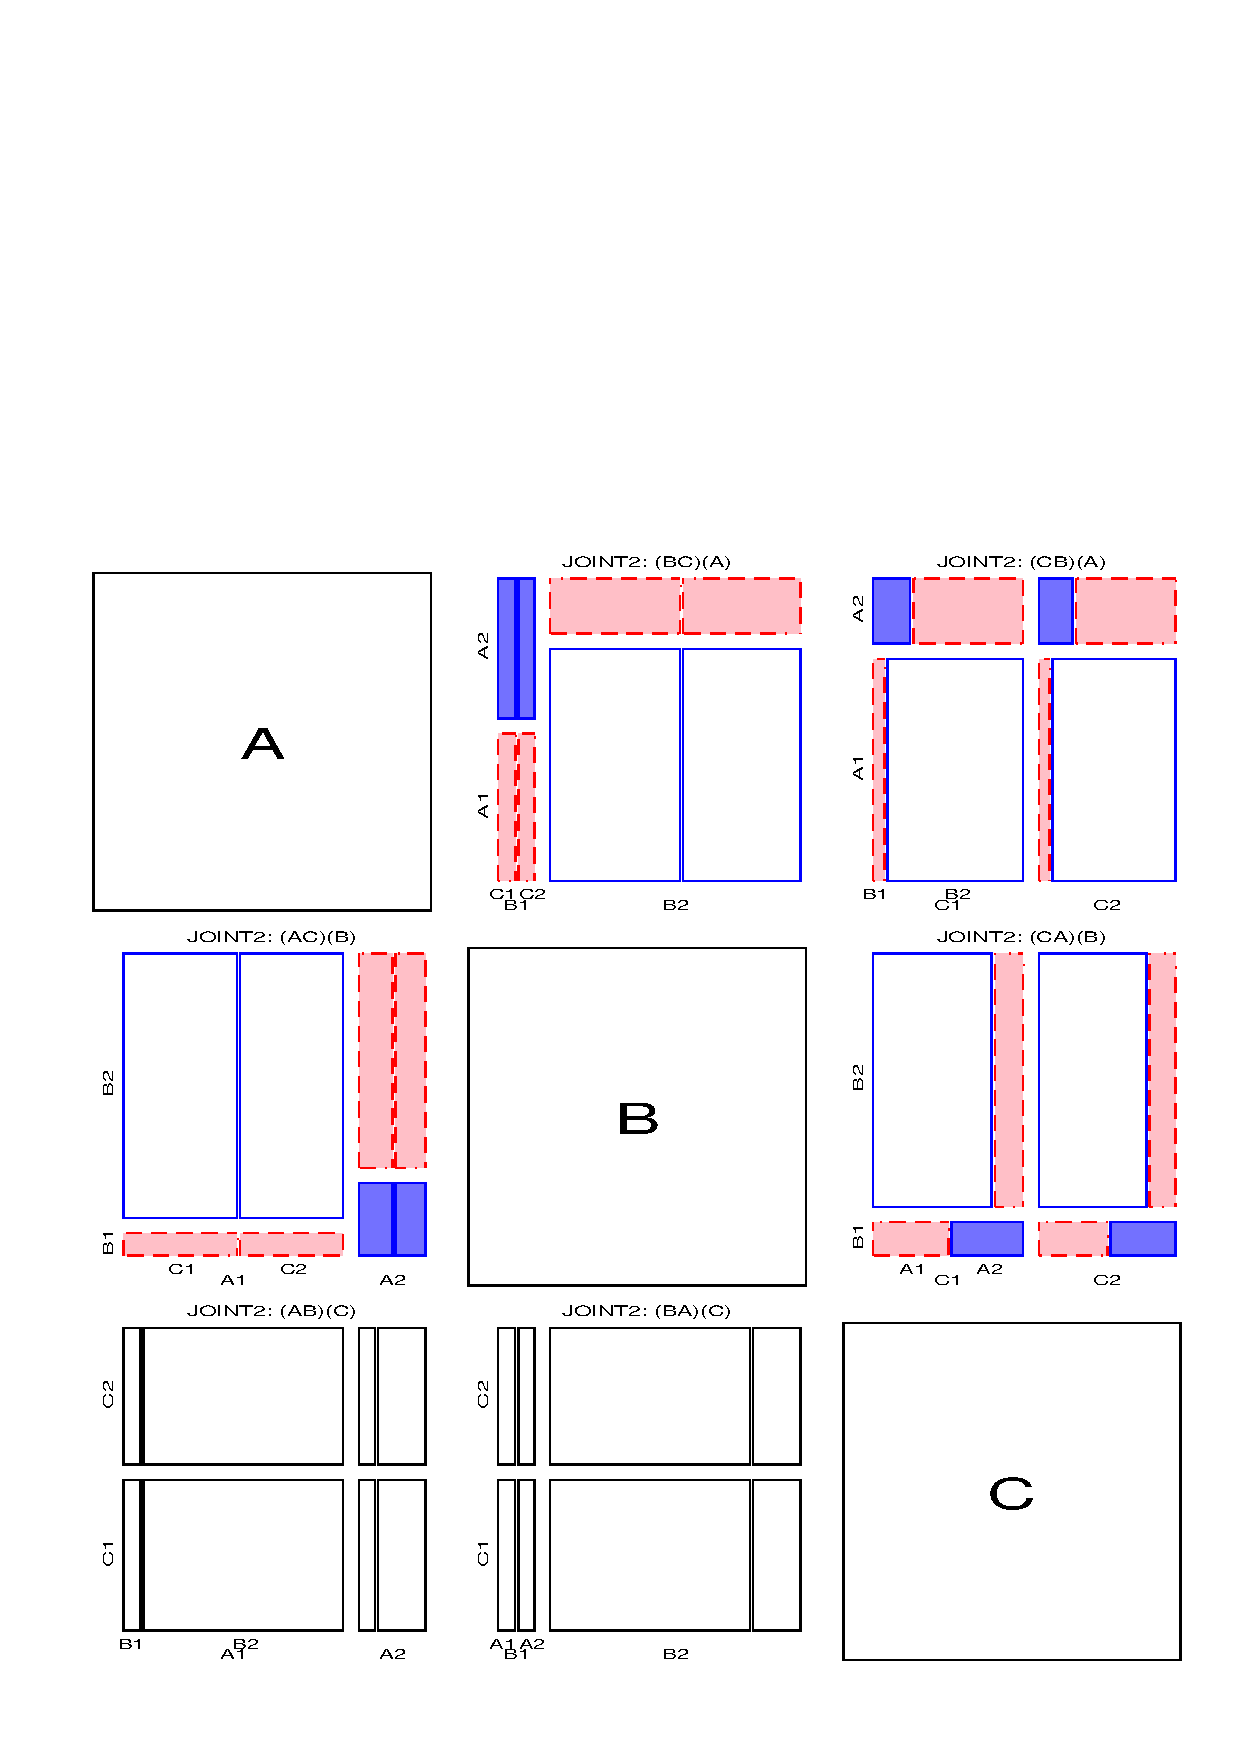
\includegraphics[scale=.6]{ch4/fig/mosfit-21}
  \caption[Mosaic matrix for joint independence]{Mosaic matrix for joint independence.  The bottom row shows that $A$ and $B$ are each independent
 of $C$, and  also
conditionally independent of $C$}%
  \label{fig:mosfit-21}
\end{figure}
\begin{verbatim}
   ...
   config = t({1 2, 3 0});
   call ipf(fit,status,dim,table,config);
   fittype='JOINT2';
   ...
\end{verbatim}
which gives these fitted frequencies.
\begin{output}
   FITTYPE  CONFIG        FIT
   JOINT2      1   3    22.59   21.54  264.81   63.05
               2   0    20.41   19.46  239.19   56.95
\end{output}
The \texttt{fittype='JOINT2';} specifies that in each panel the fitted model
is that wherein the first and third variable are independent of the second.
Now, in \figref{fig:mosfit-21}, the same model is fit in both panels in
each row,  but the second, distinguished variable differs from
row to row.

We see in row 3, where $C$ is the second variable, that $C$ is independent
of $A$, and also independent of $B$, and these models have residuals
equal to zero.
The models fit in the other four panels have non-zero residuals.
However, the $(1, 2)$ and $(2, 1)$ panels show that
$B \perp C \given A$, and $A \perp C \given B$, respectively, because
the top and bottom portions are both divided equally by the third table
variable.
This relation does not hold, however, in the $(1, 3)$ and $(2, 3)$ panels.
Thus, joint independence implies that conditional independence hold
as well, but only for the two variables which enter jointly.

The appearance in the bottom row of \figref{fig:mosfit-21}
that $A$ and $B$ are marginally independent, is
misleading, because the $AB$ association is fit exactly in these models.
To see the marginal relations under $[A B][C]$ explicitly,
we can just change the \texttt{plots} value to \texttt{plots=2;},
so that the model of (marginal) independence is fit to the first two
variables in each panel and only these variables are displayed.
This plot appears in \figref{fig:mosfit-22}, and shows
clearly that $A$ and $B$ are each marginally independent of $C$,
but not of each other.
\begin{figure}[htb]
  \centering
  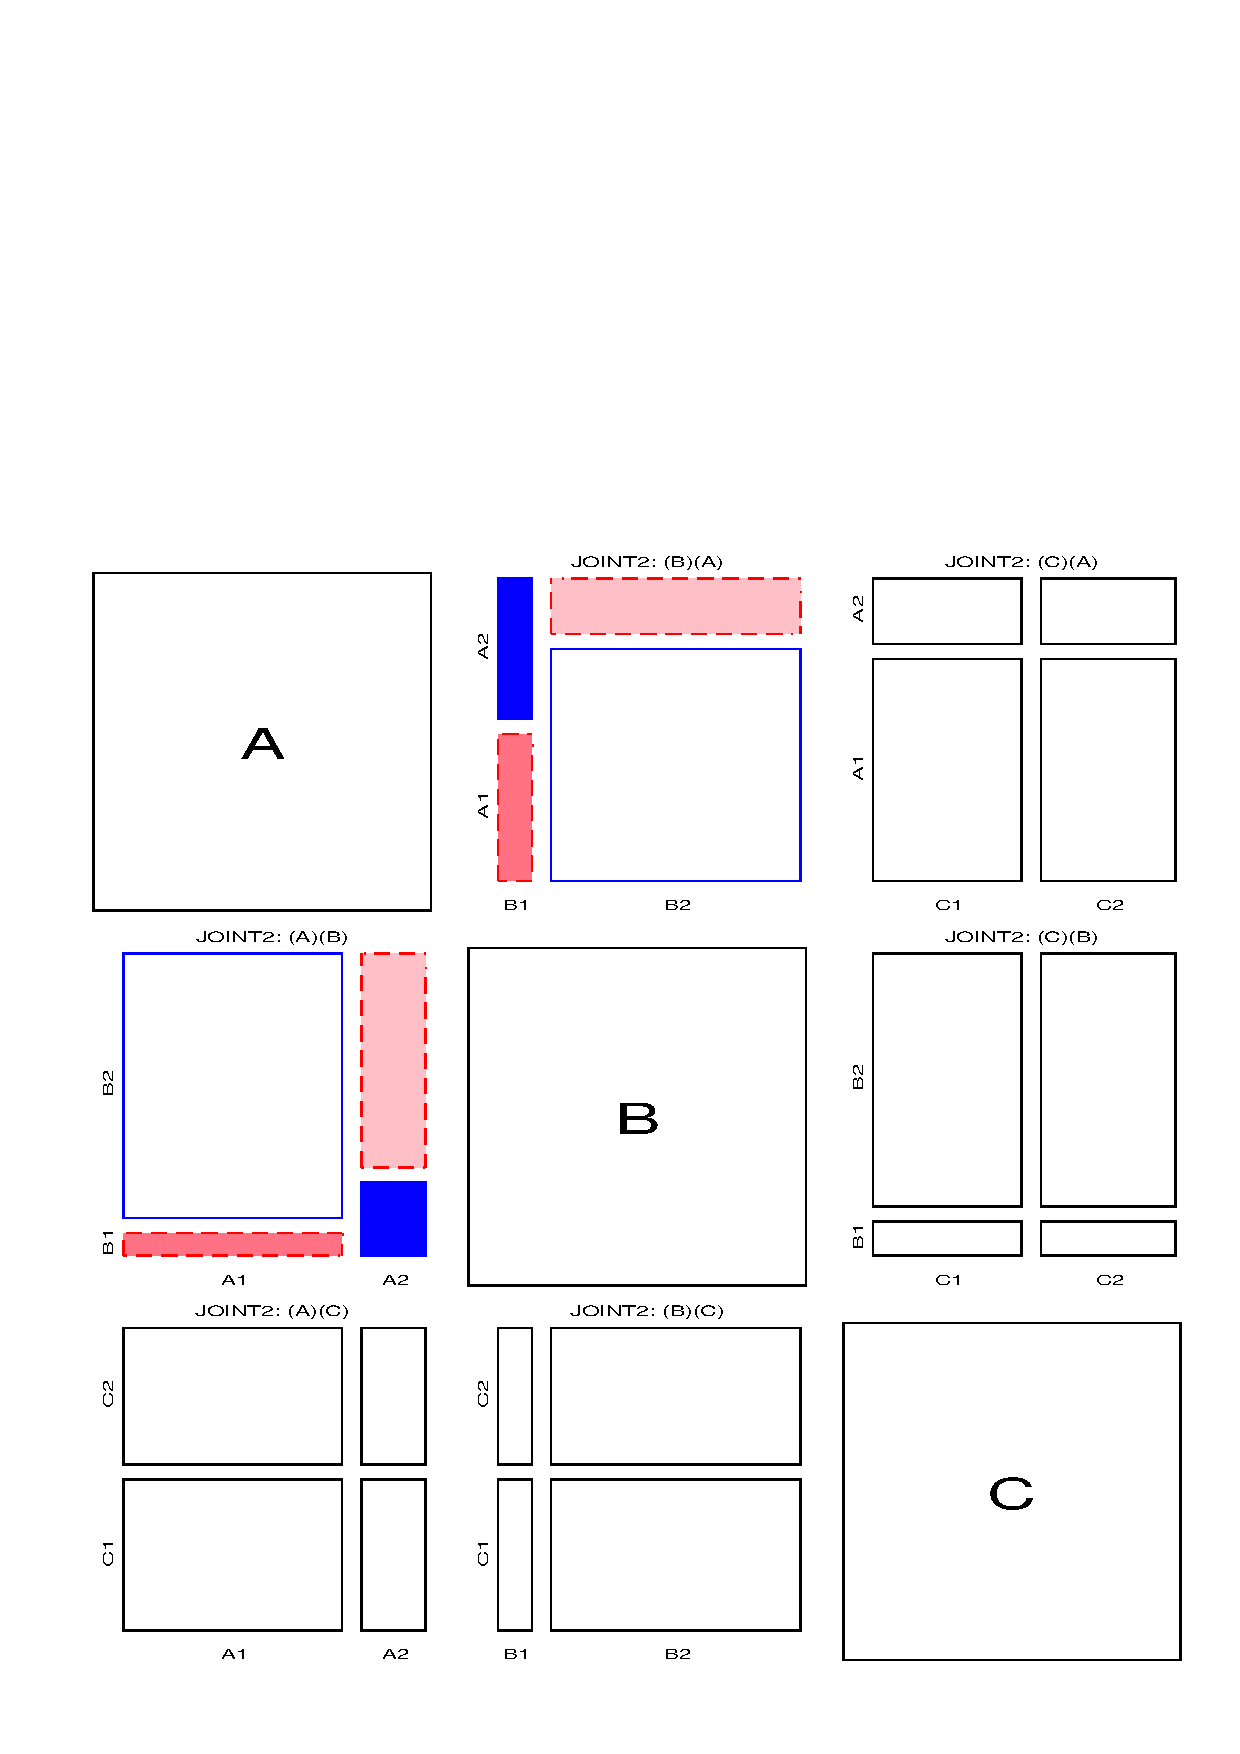
\includegraphics[scale=.6]{ch4/fig/mosfit-22}
  \caption[Marginal relations under joint independence]{Marginal relations under joint independence.  $A$ and $B$ are each marginally independent
 of $C$}%
  \label{fig:mosfit-22}
\end{figure}

\subsection{Conditional independence}
For conditional independence, $H_3: \: A  \perp B \given C$,
or $[A C][B C]$, we proceed similarly,  using
\begin{verbatim}
   config = t({1 2, 2 3});
   call ipf(fit,status,dim,table,config);
   fittype='CONDIT1';
   ...
\end{verbatim}
to obtain frequencies which fit this model exactly.
The resulting three-way mosaic matrix is shown in \figref{fig:mosfit-3}.
\begin{figure}[htb]
  \centering
  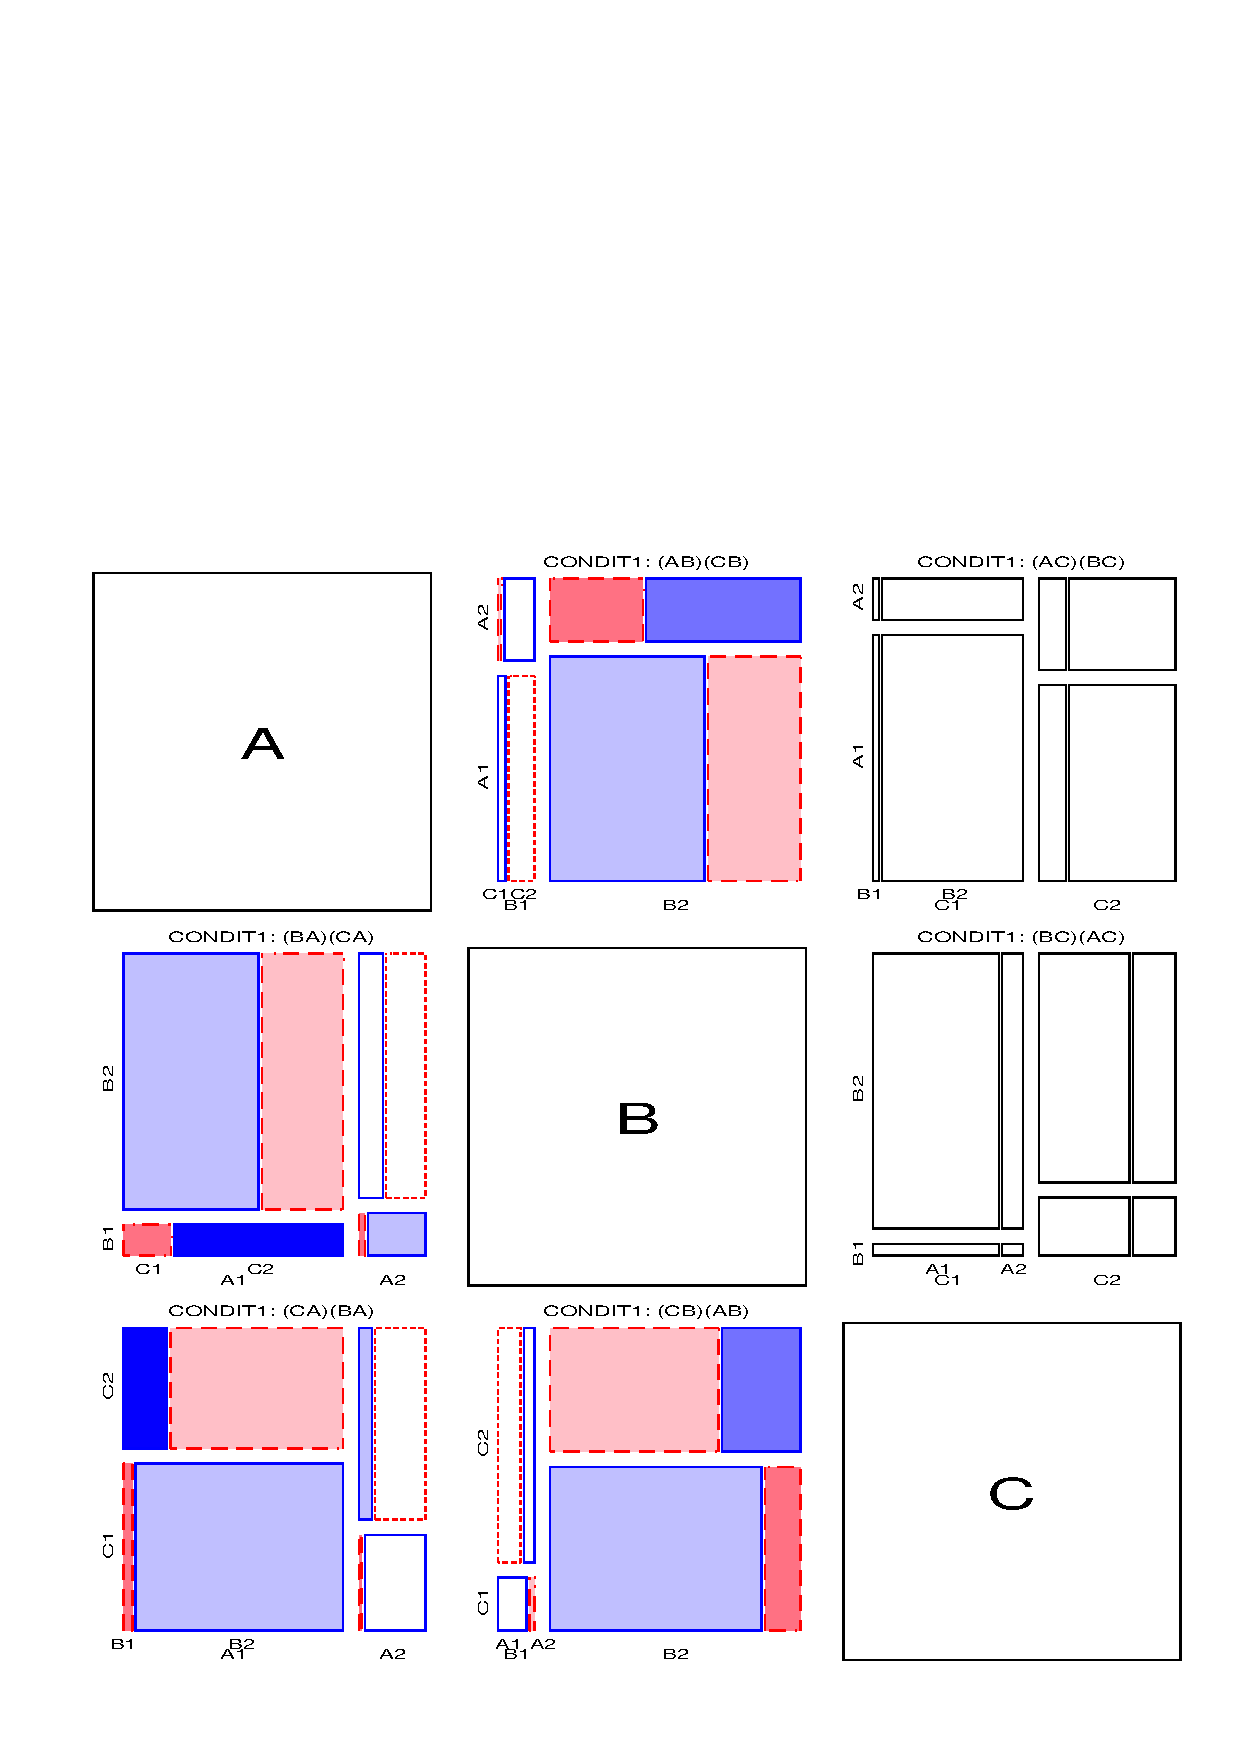
\includegraphics[scale=.6]{ch4/fig/mosfit-3}
  \caption[Mosaic matrix for conditional independence]{Mosaic matrix for conditional independence}%
  \label{fig:mosfit-3}
\end{figure}
We now see the characteristic signature of conditional independence in the
$(1, 3)$ and $(2, 3)$ panels, where $A$ and $B$ are independent at
each level of $C$. But no independence relations appear in the four
large blocks of the first two variables in any panel, so
no pair of variables is marginally independent.%
\footnote{In this data $A$ and $B$ have quite a weak association, as
may be seen in the $(1, 2)$ and $(2, 1)$ panels, where the large blocks
nearly align.}
